\tikzset{every picture/.style={line width=0.2pt}} %set default line width to 0.75pt        


\begin{tikzpicture}[x=0.75pt,y=0.75pt,yscale=-1,xscale=1]
%uncomment if require: 
\path (0,446); %set diagram left start at 0, and has height of 446
%Shape: Rectangle [id:dp03411876837432981] 
\draw[fill={rgb, 255:red, 30; green, 164; blue, 247 }  ,fill opacity=0.36 ] (13,71.03) -- (225.26,71.03) -- (225.26,244.73) -- (13,244.73) -- cycle ;
%Shape: Triangle [id:dp9375754488130867] 
\draw  [fill={rgb, 255:red, 208; green, 2; blue, 27 }  ,fill opacity=1 ] (126.3,85.43) -- (147.81,120.93) -- (104.79,120.93) -- cycle ;
%Shape: Ellipse [id:dp16442697541796703] 
\draw  [fill={rgb, 255:red, 74; green, 144; blue, 226 }  ,fill opacity=1 ] (133.47,153.08) .. controls (133.47,142.22) and (142.25,133.41) .. (153.07,133.41) .. controls (163.9,133.41) and (172.67,142.22) .. (172.67,153.08) .. controls (172.67,163.95) and (163.9,172.76) .. (153.07,172.76) .. controls (142.25,172.76) and (133.47,163.95) .. (133.47,153.08) -- cycle ;
%Shape: Ellipse [id:dp8929359456575365] 
\draw  [fill={rgb, 255:red, 74; green, 144; blue, 226 }  ,fill opacity=1 ] (23.52,153.08) .. controls (23.52,142.22) and (32.29,133.41) .. (43.12,133.41) .. controls (53.94,133.41) and (62.72,142.22) .. (62.72,153.08) .. controls (62.72,163.95) and (53.94,172.76) .. (43.12,172.76) .. controls (32.29,172.76) and (23.52,163.95) .. (23.52,153.08) -- cycle ;
%Shape: Triangle [id:dp7376655464767954] 
\draw  [fill={rgb, 255:red, 208; green, 2; blue, 27 }  ,fill opacity=1 ] (61.28,85.43) -- (82.8,120.93) -- (39.77,120.93) -- cycle ;
%Shape: Rectangle [id:dp12169534238909918] 
\draw  [fill={rgb, 255:red, 245; green, 166; blue, 35 }  ,fill opacity=1 ] (160.24,88.31) -- (199.44,88.31) -- (199.44,127.65) -- (160.24,127.65) -- cycle ;
%Shape: Rectangle [id:dp008860357027288712] 
\draw  [fill={rgb, 255:red, 245; green, 166; blue, 35 }  ,fill opacity=1 ] (165.02,184.27) -- (204.22,184.27) -- (204.22,223.62) -- (165.02,223.62) -- cycle ;
%Shape: Rectangle [id:dp9615704991146319] 
\draw  [fill={rgb, 255:red, 245; green, 166; blue, 35 }  ,fill opacity=1 ] (77.54,134.37) -- (116.74,134.37) -- (116.74,173.72) -- (77.54,173.72) -- cycle ;
%Shape: Triangle [id:dp3026521490627023] 
\draw  [fill={rgb, 255:red, 208; green, 2; blue, 27 }  ,fill opacity=1 ] (124.39,184.27) -- (145.9,219.78) -- (102.88,219.78) -- cycle ;
%Shape: Ellipse [id:dp47582021898019566] 
\draw  [fill={rgb, 255:red, 74; green, 144; blue, 226 }  ,fill opacity=1 ] (39.77,204.91) .. controls (39.77,194.04) and (48.55,185.23) .. (59.37,185.23) .. controls (70.2,185.23) and (78.97,194.04) .. (78.97,204.91) .. controls (78.97,215.77) and (70.2,224.58) .. (59.37,224.58) .. controls (48.55,224.58) and (39.77,215.77) .. (39.77,204.91) -- cycle ;
%Shape: Rectangle [id:dp29141062253976635] 
\draw  [fill={rgb, 255:red, 247; green, 204; blue, 30 }  ,fill opacity=0.36 ] (14.91,278.32) -- (227.17,278.32) -- (227.17,374.29) -- (14.91,374.29) -- cycle ;
%Shape: Ellipse [id:dp4851406617475926] 
\draw  [fill={rgb, 255:red, 74; green, 144; blue, 226 }  ,fill opacity=1 ] (100.96,312.39) .. controls (100.96,301.52) and (109.74,292.72) .. (120.56,292.72) .. controls (131.39,292.72) and (140.16,301.52) .. (140.16,312.39) .. controls (140.16,323.25) and (131.39,332.06) .. (120.56,332.06) .. controls (109.74,332.06) and (100.96,323.25) .. (100.96,312.39) -- cycle ;
%Shape: Triangle [id:dp1307613946933155] 
\draw  [fill={rgb, 255:red, 208; green, 2; blue, 27 }  ,fill opacity=1 ] (64.15,292.72) -- (85.66,328.22) -- (42.64,328.22) -- cycle ;
%Shape: Rectangle [id:dp35663833636935394] 
\draw  [fill={rgb, 255:red, 245; green, 166; blue, 35 }  ,fill opacity=1 ] (165.98,293.67) -- (205.18,293.67) -- (205.18,333.02) -- (165.98,333.02) -- cycle ;
%Straight Lines [id:da6673185348400361] 
\draw    (263.82,213.55) -- (298.82,213.5) ;
\draw [shift={(300.82,213.49)}, rotate = 179.91] [color={rgb, 255:red, 0; green, 0; blue, 0 }  ][line width=0.75]    (10.93,-3.29) .. controls (6.95,-1.4) and (3.31,-0.3) .. (0,0) .. controls (3.31,0.3) and (6.95,1.4) .. (10.93,3.29)   ;
%Straight Lines [id:da17452505371177662] 
\draw    (227,322.73) -- (263.54,323.73) ;
%Straight Lines [id:da19470043848262208] 
\draw    (226.21,149.72) -- (264.67,150.72) ;
%Straight Lines [id:da10397627231220286] 
\draw    (264.67,150.72) -- (263.54,323.73) ;
%Shape: Ellipse [id:dp8385531363983802] 
\draw  [fill={rgb, 255:red, 80; green, 227; blue, 194 }  ,fill opacity=0.49 ] (300.82,213.49) .. controls (300.82,180.48) and (341.79,153.71) .. (392.32,153.71) .. controls (442.86,153.71) and (483.82,180.48) .. (483.82,213.49) .. controls (483.82,246.51) and (442.86,273.28) .. (392.32,273.28) .. controls (341.79,273.28) and (300.82,246.51) .. (300.82,213.49) -- cycle ;
%Straight Lines [id:da2475999051951534] 
\draw    (483.82,213.49) -- (526.82,213.29) ;
\draw [shift={(528.82,213.28)}, rotate = 179.73] [color={rgb, 255:red, 0; green, 0; blue, 0 }  ][line width=0.75]    (10.93,-3.29) .. controls (6.95,-1.4) and (3.31,-0.3) .. (0,0) .. controls (3.31,0.3) and (6.95,1.4) .. (10.93,3.29)   ;
%Shape: Rectangle [id:dp03611177475200367] 
\draw  [fill={rgb, 255:red, 30; green, 164; blue, 247 }  ,fill opacity=0.36 ] (493.91,313.59) -- (664.82,313.59) -- (664.82,376.82) -- (493.91,376.82) -- cycle ;
%Shape: Triangle [id:dp8126894821695971] 
\draw  [fill={rgb, 255:red, 208; green, 2; blue, 27 }  ,fill opacity=1 ] (514.8,330.86) -- (530.82,360.28) -- (498.77,360.28) -- cycle ;
%Shape: Rectangle [id:dp7704102629126468] 
\draw  [fill={rgb, 255:red, 245; green, 166; blue, 35 }  ,fill opacity=1 ] (587.24,330.74) -- (611.82,330.74) -- (611.82,357.28) -- (587.24,357.28) -- cycle ;
%Shape: Ellipse [id:dp8221231723533802] 
\draw  [fill={rgb, 255:red, 74; green, 144; blue, 226 }  ,fill opacity=1 ] (540.96,346) .. controls (540.96,337) and (548.32,329.72) .. (557.39,329.72) .. controls (566.47,329.72) and (573.82,337) .. (573.82,346) .. controls (573.82,354.99) and (566.47,362.28) .. (557.39,362.28) .. controls (548.32,362.28) and (540.96,354.99) .. (540.96,346) -- cycle ;
%Shape: Ellipse [id:dp6362055661503672] 
\draw  [fill={rgb, 255:red, 74; green, 144; blue, 226 }  ,fill opacity=1 ] (622.82,343.78) .. controls (622.82,335.22) and (629.54,328.28) .. (637.82,328.28) .. controls (646.11,328.28) and (652.82,335.22) .. (652.82,343.78) .. controls (652.82,352.34) and (646.11,359.28) .. (637.82,359.28) .. controls (629.54,359.28) and (622.82,352.34) .. (622.82,343.78) -- cycle ;
%Rounded Rect [id:dp4276999307253777] 
\draw  [fill={rgb, 255:red, 189; green, 16; blue, 224 }  ,fill opacity=0.24 ] (530,191.88) .. controls (530,183.26) and (536.98,176.28) .. (545.6,176.28) -- (612.22,176.28) .. controls (620.84,176.28) and (627.82,183.26) .. (627.82,191.88) -- (627.82,238.68) .. controls (627.82,247.29) and (620.84,254.28) .. (612.22,254.28) -- (545.6,254.28) .. controls (536.98,254.28) and (530,247.29) .. (530,238.68) -- cycle ;
%Straight Lines [id:da16188474121366347] 
\draw    (580,314) -- (580.79,256.19) ;
\draw [shift={(580.82,254.19)}, rotate = 90.79] [color={rgb, 255:red, 0; green, 0; blue, 0 }  ][line width=0.75]    (10.93,-3.29) .. controls (6.95,-1.4) and (3.31,-0.3) .. (0,0) .. controls (3.31,0.3) and (6.95,1.4) .. (10.93,3.29)   ;
%Straight Lines [id:da6849788730551594] 
\draw    (628.41,211.78) -- (667.82,211.82) ;
\draw [shift={(669.82,211.82)}, rotate = 180.05] [color={rgb, 255:red, 0; green, 0; blue, 0 }  ][line width=0.75]    (10.93,-3.29) .. controls (6.95,-1.4) and (3.31,-0.3) .. (0,0) .. controls (3.31,0.3) and (6.95,1.4) .. (10.93,3.29)   ;
%Shape: Cube [id:dp11030403935801325] 
\draw  [fill={rgb, 255:red, 155; green, 155; blue, 155 }  ,fill opacity=1 ] (669,192.65) -- (688.01,173.64) -- (735.82,173.64) -- (735.82,217.99) -- (716.81,237) -- (669,237) -- cycle ; \draw   (735.82,173.64) -- (716.81,192.65) -- (669,192.65) ; \draw   (716.81,192.65) -- (716.81,237) ;
%Shape: Triangle [id:dp48891639752656224] 
\draw  [fill={rgb, 255:red, 208; green, 2; blue, 27 }  ,fill opacity=0.74 ] (693.82,204.64) -- (704.82,223.28) -- (682.77,223.28) -- cycle ;
%Shape: Ellipse [id:dp8314174152258622] 
\draw  [fill={rgb, 255:red, 74; green, 144; blue, 226 }  ,fill opacity=0.61 ] (692.68,182.96) .. controls (695.97,179.47) and (703.99,176.64) .. (710.59,176.64) .. controls (717.19,176.64) and (719.86,179.47) .. (716.57,182.96) .. controls (713.27,186.45) and (705.25,189.28) .. (698.66,189.28) .. controls (692.06,189.28) and (689.38,186.45) .. (692.68,182.96) -- cycle ;
%Shape: Rectangle [id:dp03254240217615467] 
\draw  [fill={rgb, 255:red, 245; green, 166; blue, 35 }  ,fill opacity=0.55 ] (720.08,200.39) -- (732.82,188.28) -- (732.38,210.57) -- (719.65,222.67) -- cycle ;

% Text Node
\draw (291,9) node [anchor=north west][inner sep=0.75pt]   [align=left] {{\fontfamily{helvet}\selectfont {\Large Supervised Learning}}};
% Text Node
\draw (74.98,48.58) node [anchor=north west][inner sep=0.75pt]   [align=left] {Training Data};
% Text Node
\draw (92.3,379.7) node [anchor=north west][inner sep=0.75pt]   [align=left] {Labels};
% Text Node
\draw (40.7,341.4) node [anchor=north west][inner sep=0.75pt]  [font=\footnotesize] [align=left] {Triangle};
% Text Node
\draw (100.26,340.44) node [anchor=north west][inner sep=0.75pt]  [font=\footnotesize] [align=left] {Circle};
% Text Node
\draw (165.08,341.4) node [anchor=north west][inner sep=0.75pt]  [font=\footnotesize] [align=left] {Square};
% Text Node
\draw (330,177.4) node [anchor=north west][inner sep=0.75pt]    {$ \begin{array}{l}
\ \ \ \ \ f_{i}(\textcolor[rgb]{0.82,0.01,0.11}{\blacktriangle }) =\ \hat{y}\\
\mathcal{L}( y,\ \hat{y}) \ \rightarrow f_{i+1} \ 
\end{array}$};
% Text Node
\draw (312,123) node [anchor=north west][inner sep=0.75pt]   [align=left] {{\Large \faCog}};
% Text Node
\draw (341.98,125.58) node [anchor=north west][inner sep=0.75pt]   [align=left] {Model Training};
% Text Node
\draw (449,122) node [anchor=north west][inner sep=0.75pt]   [align=left] {{\Large \faCog}};
% Text Node
\draw (340,235) node [anchor=north west][inner sep=0.75pt]   [align=left] {{\footnotesize Learning algorithm}};
% Text Node
\draw (551.98,386.01) node [anchor=north west][inner sep=0.75pt]   [align=left] {Test Data};
% Text Node
\draw (520,132) node [anchor=north west][inner sep=0.75pt]   [align=left] {\begin{minipage}[lt]{86.41pt}\setlength\topsep{0pt}
\begin{center}
{\small Model }\\{\small Inference/Evaluation}
\end{center}

\end{minipage}};
% Text Node
\draw (533,193) node [anchor=north west][inner sep=0.75pt]   [align=left] {$\displaystyle f(\textcolor[rgb]{0.82,0.01,0.11}{\blacktriangle })$};
% Text Node
\draw (572,194) node [anchor=north west][inner sep=0.75pt]   [align=left] {{\scriptsize = Triangle?}};
% Text Node
\draw (543.82,220.28) node [anchor=north west][inner sep=0.75pt]   [align=left] {{\scriptsize \textcolor[rgb]{0.29,0.29,0.29}{metric = 0.999 }}};
% Text Node
\draw (668.98,152.01) node [anchor=north west][inner sep=0.75pt]   [align=left] {Final Model};
% Text Node
\draw (653,249) node [anchor=north west][inner sep=0.75pt]   [align=left] {$\displaystyle f(\textcolor[rgb]{0.82,0.01,0.11}{\blacktriangle ,}\textcolor[rgb]{0.29,0.56,0.89}{\bullet} ,\textcolor[rgb]{0.96,0.65,0.14}{\blacksquare }) \tiny{=\{label\}}$  };

\end{tikzpicture}

